\documentclass[10pt]{standalone}
\usepackage{tikz}
\usetikzlibrary{
  calc,
  patterns,
  decorations.pathmorphing,
}





\begin{document}

\noindent
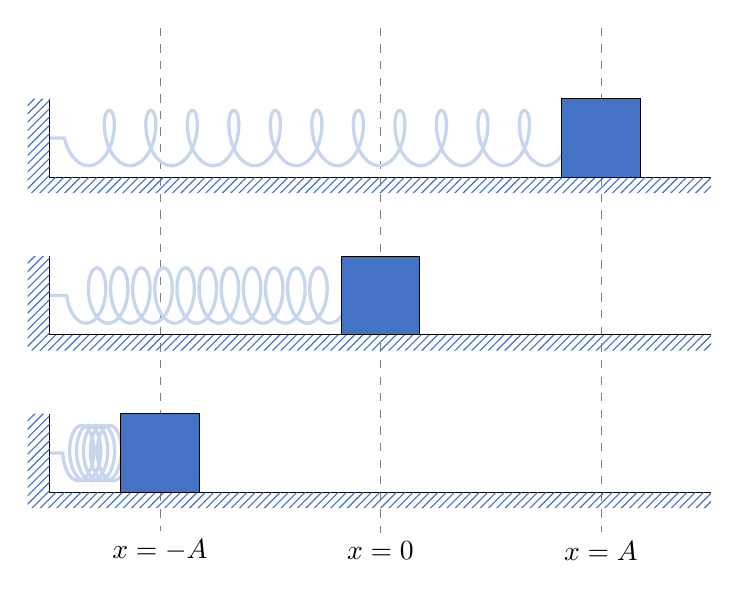
\begin{tikzpicture}
  \def\amp{2.8}
  \def\massradius{.5}
  \def\sep{2}
  \def\ceilingheight{2*\amp}
  \def\startofspring{1.7*\amp}
  \def\endofpicx{\startofspring+3.5*\sep}
  \def\endofpicy{-10}
  \def\springending{.1}
  \def\veclength{1.25}
  \def\leftanchor{-1.5*\amp}

  \definecolor{springcolor}{HTML}{4472C4}
  \definecolor{circlecolor}{HTML}{C5DFB5}

  \tikzstyle{guides}=[
      ultra thin,
      gray,
      dashed
    ]
  \tikzstyle{smass}=[
      %radius=\massradius,
      fill=springcolor,
    ]
  \tikzstyle{ceiling}=[
      pattern=north east lines,
      pattern color=springcolor
    ]
  \tikzstyle{spring}=[
      very thick,
      springcolor!30,
      decoration={
        coil,
        amplitude=10
      }
    ]
  \tikzstyle{vector}=[
      red!30,
      very thick,
      ->
    ]

  \coordinate (ceiling start) 
                  at (\leftanchor, -0.5*\amp);
  \coordinate (ceiling end)   
                  at (\leftanchor, \endofpicy);
  %\fill[ceiling] (ceiling start) -- (ceiling end)
  %   -- ++(-.5,0) |- cycle;
  %\draw (ceiling start) -- (ceiling end) -- ++ (-0.5,0);

  \draw[guides] (-\amp, -1.2*\amp) -- (-\amp, \endofpicy);
  \draw[guides] ( \amp, -1.2*\amp) -- ( \amp, \endofpicy);
  \draw[guides] (0    , -1.2*\amp) -- (0    , \endofpicy);



  

  \path[smass]
      (\amp ,-\startofspring) coordinate (s1)
    ++(-\amp,  -\sep) coordinate (s3)
    ++(-\amp,  -\sep) coordinate (s4);

  \node[fill=white] at (0,\endofpicy) {$x=0$};
  \node[fill=white] at (\amp,\endofpicy) {$x=A$};
  \node[fill=white] at (-\amp,\endofpicy) {$x=-A$};




  %usage \drawspring{(location of mass)}{segment length}
  \newcommand{\drawspring}[2]{
    \coordinate (thismass) at #1;
    \coordinate (top) at 
      (ceiling start |- thismass);
    \draw[spring,segment length=#2] (thismass)
      -- ++ (-\massradius+\springending,0) 
      decorate {-- ($(top) + (\springending,0)$) }
      -- (top);
    \draw (top) +(0,0.5) -- ++(0,-0.5) -- ++(3*\amp,0);
    \fill[ceiling] 
      (top) +(0,0.5) -- ++(0,-0.5) -- ++(3*\amp,0)
      -- ++(0,-0.2) -- ++(-3.1*\amp,0) 
      -- ++(0,1.2) -- cycle;
  }

  \drawspring{(s1)}{15}
  \draw[smass] (s1) +(\massradius,\massradius) rectangle +(-\massradius,-\massradius);

  \drawspring{(s3)}{8}
  \draw[smass] (s3) +(\massradius,\massradius) rectangle +(-\massradius,-\massradius);

  \drawspring{(s4)}{2.5}
  \draw[smass] (s4) +(\massradius,\massradius) rectangle +(-\massradius,-\massradius);



\end{tikzpicture}




\end{document}